% !TEX root = ../main.tex

\chapter{ShiDianNao加速器架构}

如图\ref{fig:shidiannao_acc_arch}所示,我们的加速器由以下主要组件组成:输入和输出神经元的两个缓冲区(NBin和NBout)、突触的缓冲区(SB)、计算输出神经元的神经功能单元(NFU)和算术单元(ALU)以及指令的缓冲区和解码器(IB)。
在本节的其余部分中,我们将介绍计算结构,在接下来的部分中,我们将描述存储和控制结构。
我们的加速器有两个功能单元,一个NFU调节基本神经元操作(乘法、加法和比较)和一个ALU执行激活函数计算。
在这两种计算结构中,我们使用16位定点算术运算符,而不是传统的32位浮点运算符,原因有两方面。
首先,使用16位定点算子会给神经网络带来可忽略不计的精度损失,这已被先前的研究所验证。
其次,使用较小的运营商可以显著降低硬件成本。例如,在台积电65nm技术中,16位截断定点乘法器比32位浮点多乘法器小6.10倍,节能7.33倍.

\begin{figure}[htbp]
  \centering
  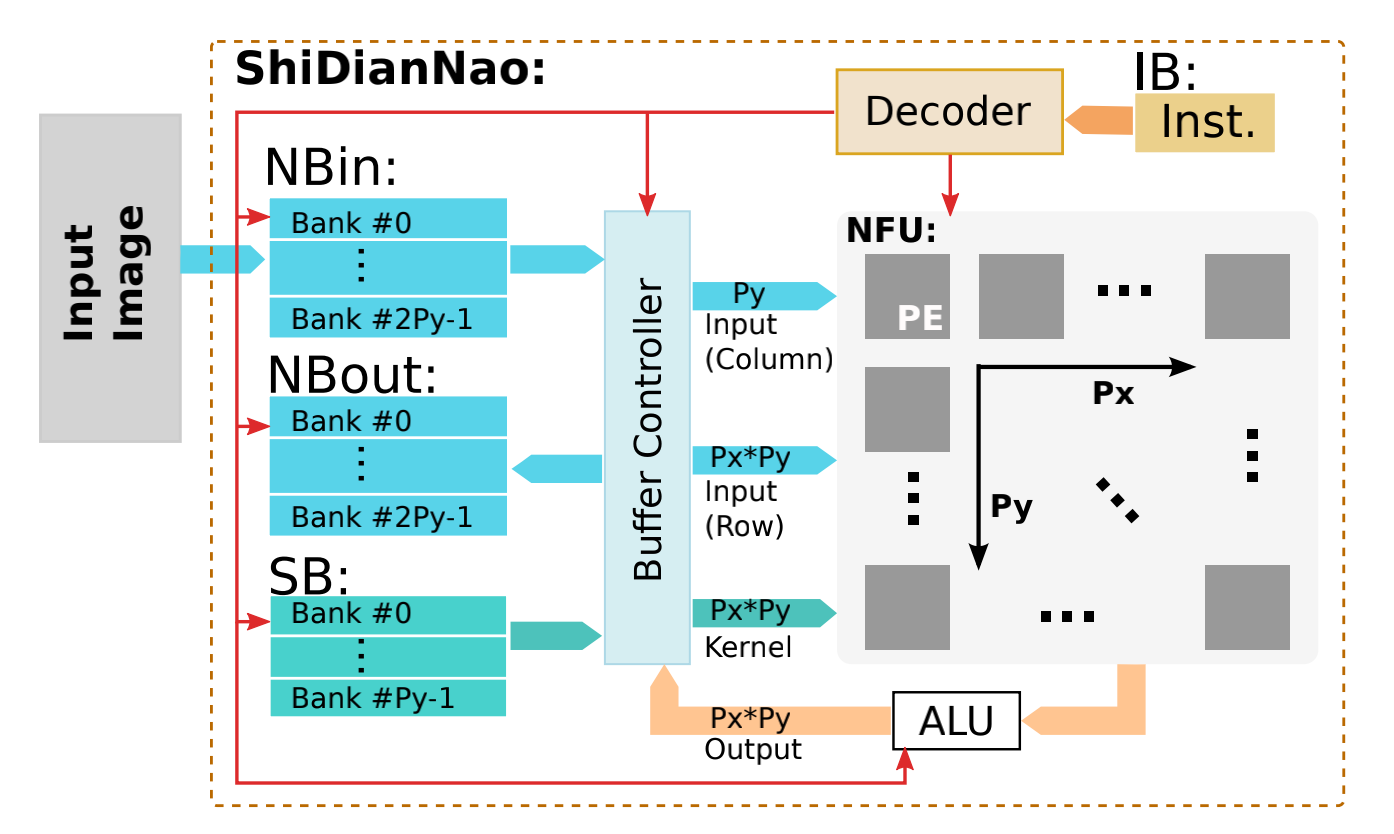
\includegraphics[width=12cm]{figures/shidiannao_acc_arch.png}
  \caption{ShiDianNao加速器架构图}
  \label{fig:shidiannao_acc_arch}
\end{figure} 

